\section{Model}
\subsection{Problem Overview} In this article, we are going to estimate the maximum windspeed that allows the quadcopter to stay within 20cm from the target. We will first simplify the quadcopter dynamics model to reduce the calculation complexity in algorithm. Based on the rigid body dynamics, we then derive equations of motions and then use python to build a physical simulation system for the quadcopter. We then develop a thrust control system that can control the quadcopter to react to the wind and maintain its stability. By inputting basically two patterns of wind(periodic and noise) into our simulation with different magnitude, we run the simulation repeatly and get the average time that the quadcopter is able to stay within desired range. If the time is large enough, the corresponding windspeed is allowed for the safe operation. The maximum windspeed can be found accordingly.

\begin{figure}[htbp]
\centering
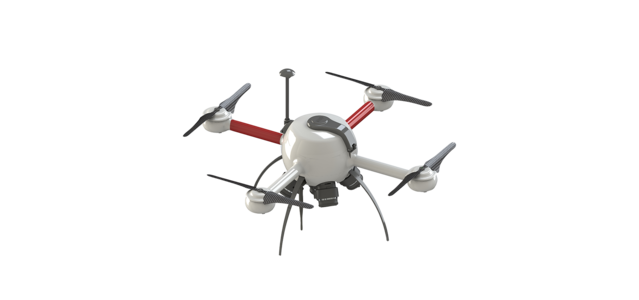
\includegraphics[width= 0.7\linewidth, angle =0]{Images/quadcopter.png}
\caption{Quadcopter overview.}
\label{fig:1}
\end{figure}

\subsection{Assumption and Definition}
\subsubsection{Quadcopter model simplification}
The drone we used in our model has a total mass of $1.5 $kg, and is powered by four rotors which can each generate a thrust up to $7$ N.

The major mass of the quadcopter is concentrated on the platform in the middle. Therefore, in order to simplify the dynamics equation of motion during the operation of the quadcopter, we assume that the platform in the center is a homogeneous sphere with a radius $r=10cm$ and a mass $m=1kg$. Four rotors are arranged in a square, each with a mass $m_{r}=0.125kg$, and a distance of $d = 50cm$ from the sphere center. We assume that the four rods connecting the rotor to the central sphere are light enough that it can be ignored in the dynamics model. The model frame is showed in Figure \ref{fig:model}.

As for staying within 20 cm, as our model, including the thrust control system algorithm, is rough, if the quadcopter is able to stay within 20 cm around the target for 30 s, it is believed that if the optimized control algorithm is given, the quadcopter can stay for as long as possible. Thus, the objective of the simulation is to find the maximum wind speed that the quadcopter can resist to stay within 20 cm around the target for 30 s.

\subsubsection{Aerodynamics of the model}
According to the study on the propeller aerodynamics \cite{bib1}, the aerodynamic effects applied to the rotor are evaluated by integrating, along each rotor blade, the aerodynamic force per surface increment.

By integrating the lift per surface increment, we obtain the lift force LF (or thrust)
\begin{equation}
 \mathbf{F_{L}}=\rho c R^{3} \omega^{2} C_{L \alpha}\left(\frac{\alpha_{0}}{3}-\frac{\bar{w}+L\left(\varepsilon_{1} q-\varepsilon_{2} p\right)}{2 R|\omega|}\right) \hat{\mathbf{z}_{\mathbf{B}}}
\end{equation}
where $R$ is the radius of the rotor blade, $\rho$ is the air density, $U$ is the airspeed, $c$ is the blade width, $C_{L \alpha}$ is the lift coefficient, $\alpha_{0}$ its pitch angle at rest. The coefficients $\varepsilon_{1}$ and $\varepsilon_{2}$ depend on the rotor under consideration.

The first item with $\omega^{2}$ is far more larger than other items. Thus, the equation for the lift force can be safely reduced to \begin{equation}
\mathbf{F_{L}}=\frac{1}{3}\rho c R^{3} \omega^{2} C_{L \alpha}\alpha_{0} \hat{\mathbf{z}_{\mathbf{B}}}
\end{equation}

Here the lift coefficient $C_{L\alpha}$ can be approximate by the average pitch angle $\overline{\alpha}$ \cite{bib3} of the blade. \begin{equation}
    C_{L\alpha}=c_{l}sin(\overline{\alpha})cos(\overline{\alpha}).
\end{equation}

In our model, we set $\rho=1.225kg/m^{3}$, $c=3cm$, $R=5cm$, $\overline{\alpha}=0.78$, thus $$\mathbf{F_{L}}=0.01\omega^{2}$$.

For the drag force on the rotors, we neglect the interactions of the vehicle dynamics onto the aerodynamics effects, thus the drag force caused by the rotors is zero.

For the drag force on the middle sphere 
\begin{equation}
\label{sphereDrag}
\mathbf{F_{d}}=\frac{1}{2}\rho A \norm{\boldsymbol{u_r}} \boldsymbol{u_r} C_{d},
\end{equation}where $A=\pi r^{2}$ is the cross section area of the sphere, $\boldsymbol{u_r}=\boldsymbol{w}-\dot{\boldsymbol{\xi}}$ is the velocity of wind relative to the quadcopter in the ground frame and $C_{d}$ is the drag coefficient. Here we set $C_{d}=1.$

\subsection{Physics simulation system}

\begin{figure}[htbp]
\centering
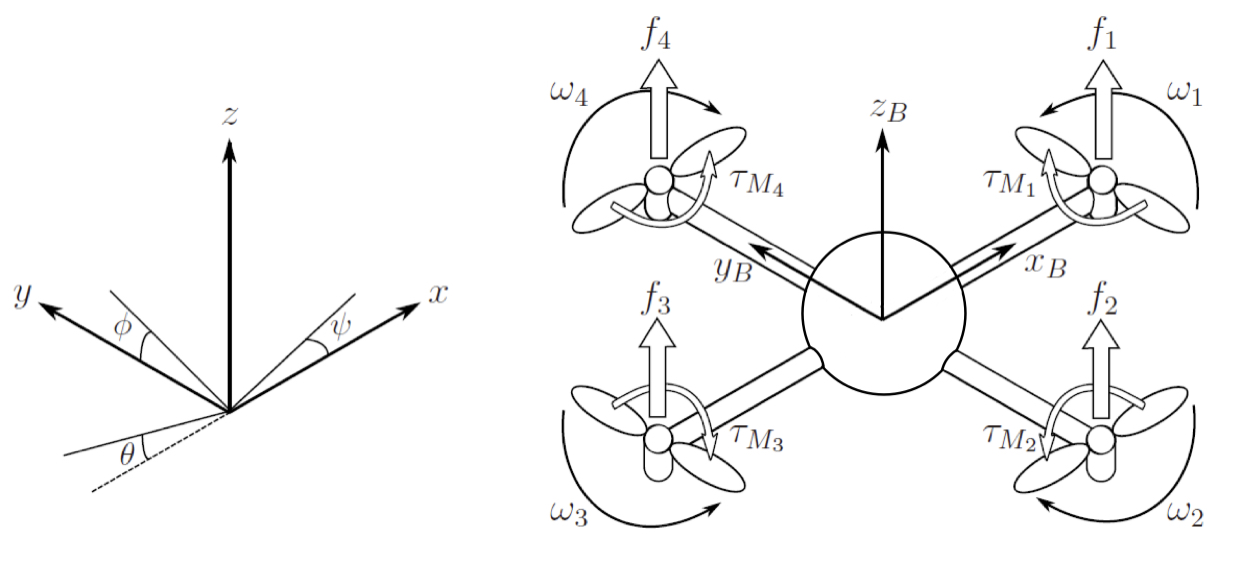
\includegraphics[width= 0.7\linewidth, angle =0]{Images/Model.png}
\caption{The simplified frame for a quadcopter.}
\label{fig:model}
\end{figure}
The dynamics of the quadcopter's motion is approached with rigid body mechanics in \cite{bib2}. We adopted notations from the paper but also made necessary simplifications to the model. The quadcopter has 6 degrees of freedom, 3 for translational motion and 3 for rotation.
Both the ground frame and the body frame are considered for solving the motion of the quadcopter. The axes of the body frame $x_B, y_B$ and $z_B$ are indicated in Figure\ref{fig:model}. The origin of the body frame is located at the center of mass of the quadcopter, which is the center of the central sphere in our model.

In the ground frame, the Cartesian coordinates $\mathrm{x}, \mathrm{y}, \mathrm{z}$ is denoted by $\boldsymbol{\xi}$. The posture of the quadcopter is described with Euler angle $\boldsymbol{\eta}$ with components $\phi, \theta$ and $\psi$, as shown in Figure\ref{fig:model}.

$$
\boldsymbol{\xi}=\left[\begin{array}{l}
x \\
y \\
z
\end{array}\right], \quad \boldsymbol{\eta}=\left[\begin{array}{l}
\phi \\
\theta \\
\psi
\end{array}\right]
$$
In the body frame, we denote the linear velocity with $\boldsymbol{V}_{B}$ and the angular velocities with $\boldsymbol{\nu}$.
$$
\boldsymbol{V}_{B}=\left[\begin{array}{l}
v_{x, B} \\
v_{y, B} \\
v_{z, B}
\end{array}\right], \quad \boldsymbol{\nu}=\left[\begin{array}{l}
p \\
q \\
r
\end{array}\right]
$$
The rotation matrix from the body frame to the inertial frame is an orthogonal matrix
$$
\boldsymbol{R}=\left[\begin{array}{ccc}
C_{\psi} C_{\theta} & C_{\psi} S_{\theta} S_{\phi}-S_{\psi} C_{\phi} & C_{\psi} S_{\theta} C_{\phi}+S_{\psi} S_{\phi} \\
S_{\psi} C_{\theta} & S_{\psi} S_{\theta} S_{\phi}+C_{\psi} C_{\phi} & S_{\psi} S_{\theta} C_{\phi}-C_{\psi} S_{\phi} \\
-S_{\theta} & C_{\theta} S_{\phi} & C_{\theta} C_{\phi}
\end{array}\right]
$$

The transformation matrix for angular velocities from the inertial frame to the body frame is $\boldsymbol{W}_{\eta},$ and from the body frame to the inertial frame is $\boldsymbol{W}_{\eta}^{-1},$ as shown in

\begin{equation}
\dot{\boldsymbol{\eta}}=\boldsymbol{W}_{\eta}^{-1} \boldsymbol{\nu}, \quad\left[\begin{array}{c}
\dot{\phi} \\
\dot{\theta} \\
\dot{\psi}
\end{array}\right]=\left[\begin{array}{ccc}
1 & S_{\phi} T_{\theta} & C_{\phi} T_{\theta} \\
0 & C_{\phi} & -S_{\phi} \\
0 & S_{\phi} / C_{\theta} & C_{\phi} / C_{\theta}
\end{array}\right]\left[\begin{array}{l}
p \\
q \\
r
\end{array}\right]
\end{equation}


\begin{equation}
\boldsymbol{\nu}=\boldsymbol{W}_{\eta} \dot{\boldsymbol{\eta}}, \quad\left[\begin{array}{c}
p \\
q \\
r
\end{array}\right]=\left[\begin{array}{ccc}
1 & 0 & -S_{\theta} \\
0 & C_{\phi} & C_{\theta} S_{\phi} \\
0 & -S_{\phi} & C_{\theta} C_{\phi}
\end{array}\right]\left[\begin{array}{c}
\dot{\phi} \\
\dot{\theta} \\
\dot{\psi}
\end{array}\right]
\end{equation}

in which $T_{x}=\tan (x)$. The matrix $\boldsymbol{W}_{\eta}$ is invertible if $\theta \neq (2 k-1) \phi / 2$, $k \in \mathbf{Z}$

In our simplified model of the quadcopter, the inertia of its body (excluding the rotors) can be obtained as the inertia of tensor of a sphere:
\begin{equation}
\boldsymbol{I} = \frac{1}{5}mr^2 \boldsymbol{I}_3
\end{equation}

The angular velocities the four rotors are denoted by $\omega_i$ ($i = 1, 2, 3, 4$). For simplicity the air drag arising from the rotation and angular acceleration of the rotors are omitted.

We use $T$ to denote the combined force given by the rotors in the $z_B$ direction. In the body frame, the combined force is
\begin{equation}
\boldsymbol{T}_{B}=\left[\begin{array}{l}
0 \\
0 \\
T
\end{array}\right]
\quad \text{where} \quad
T=\sum_{i=1}^{4} f_{i}=k \sum_{i=1}^{4} \omega_{i}^{2}
\end{equation}

Also, the torque caused by the thrust is
\begin{equation}
\boldsymbol{\tau}_{B}=\left[\begin{array}{c}
\tau_{\phi} \\
\tau_{\theta} \\
\tau_{\psi}
\end{array}\right]=\left[\begin{array}{c}
d(f_4 - f_2) \\
d(f_3 - f_1) \\
0
\end{array}\right]
\end{equation}
The physical significance of the torque is clear: by altering the difference between $f_4$ and $f_2$, rolling movement can be obtained; by altering the difference between $f_3$ and $f_1$, one can obtain pitch movement.
The acquirement of yaw movement is a little more subtle, and we'll soon notice that yaw movement arises from gyroscopic force $\Gamma$ in Newton-Euler equations.

The translational and rotational motion of the quadcopter can be fully described with Newton-Euler equations. For translational motion, it's easier to use the ground frame: 

\begin{equation}
\label{translationEquation}
m \ddot{\boldsymbol{\xi}}=\boldsymbol{G}+\boldsymbol{R} \boldsymbol{T}_{B} + \boldsymbol{F}_{\text{wind}}
\end{equation}

\begin{equation}
\left[\begin{array}{c}
\ddot{x} \\
\ddot{y} \\
\ddot{z}
\end{array}\right]=-g\left[\begin{array}{c}
0 \\
0 \\
1
\end{array}\right]+\frac{T}{m}\left[\begin{array}{c}
C_{\psi} S_{\theta} C_{\phi}+S_{\psi} S_{\phi} \\
S_{\psi} S_{\theta} C_{\phi}-C_{\psi} S_{\phi} \\
C_{\theta} C_{\phi}
\end{array}\right]
\end{equation}
where $F_{\text{wind}}$ is the drag force given in Equation\ref{sphereDrag}.
For rotational movement, we can obtain the angular acceleration with

\begin{equation}
\boldsymbol{I} \dot{\boldsymbol{\nu}}+\boldsymbol{\nu} \times(\boldsymbol{I} \boldsymbol{\nu})+\boldsymbol{\Gamma}=\boldsymbol{\tau}
\end{equation}

\begin{equation}
\label{angularEquation}
\dot{\boldsymbol{\nu}}=\boldsymbol{I}^{-1}\left(-\left[\begin{array}{c}
p \\
q \\
r
\end{array}\right] \times\left[\begin{array}{c}
I_{x x} p \\
I_{y y} q \\
I_{z z} r
\end{array}\right]-I_{r}\left[\begin{array}{c}
p \\
q \\
r
\end{array}\right] \times\left[\begin{array}{l}
0 \\
0 \\
1
\end{array}\right] \omega_{\Gamma}+\boldsymbol{\tau}\right)
\end{equation}

where $\omega_{\Gamma}=\omega_{1}-\omega_{2}+\omega_{3}-\omega_{4}$ and $I_r$ is the moment of inertia of each rotor relative to its axis of symmetry. 

With the angular acceleration in body frame obtained, we can derive that in the ground frame with $\boldsymbol{W}_{\eta}$:

\begin{equation}
\label{groundAngularAcceleration}
\begin{aligned}
\ddot{\boldsymbol{\eta}} &=\frac{\mathrm{d}}{\mathrm{d} t}\left(\boldsymbol{W}_{\eta}^{-1} \boldsymbol{\nu}\right)=\frac{\mathrm{d}}{\mathrm{d} t}\left(\boldsymbol{W}_{\eta}^{-1}\right) \boldsymbol{\nu}+\boldsymbol{W}_{\eta}^{-1} \dot{\boldsymbol{\nu}} \\
&=\left[\begin{array}{ccc}
0 & \dot{\phi} C_{\phi} T_{\theta}+\dot{\theta} S_{\phi} / C_{\theta}^{2} & -\dot{\phi} S_{\phi} C_{\theta}+\dot{\theta} C_{\phi} / C_{\theta}^{2} \\
0 & -\dot{\phi} S_{\phi} & -\dot{\phi} C_{\phi} \\
0 & \dot{\phi} C_{\phi} / C_{\theta}+\dot{\phi} S_{\phi} T_{\theta} / C_{\theta} & -\dot{\phi} S_{\phi} / C_{\theta}+\dot{\theta} C_{\phi} T_{\theta} / C_{\theta}
\end{array}\right] \boldsymbol{\nu}+\boldsymbol{W}_{\eta}^{-1} \dot{\boldsymbol{\nu}}
\end{aligned}
\end{equation}

\subsection{Thrust control system}
\label{Sec:Flight control}
Our thrust control system is designed as an linear optimization problem for $f_1, f_2, f_3, f_4$. In each step, our goal is to
\begin{itemize}
    \item maximize the component of the velocity in the direction that points to the origin.
    \item maximize the component of angular acceleration in the direction opposite to the current angular velocity.
\end{itemize}

In other words, our goal is to
    \begin{equation}
        \text{maximize  } (\dot{\boldsymbol{\xi}} + \boldsymbol{\xi} \Delta t) \cdot (- \boldsymbol{r}) \text{  subject to  } f_i \leq 7 \text{N } (i= 1, 2, 3, 4)
    \end{equation}
    and 
    \begin{equation}
        \text{maximize  } (\boldsymbol{\dot{\boldsymbol{\eta}}} + \ddot{\boldsymbol{\eta}} \Delta t) \cdot (- \boldsymbol{\eta})
        \text {  subject to } f_i \leq 7 \text{N } (i = 1, 2, 3, 4)
    \end{equation}
    
    with Equation\ref{translationEquation}, Equation\ref{angularEquation} and Equation\ref{groundAngularAcceleration} these two optimization goals can be reduced to
    \begin{equation}
        \text{minimize } (\boldsymbol{R} \boldsymbol{T}^{B}) \cdot \boldsymbol{\xi} 
    \end{equation}
    and
    \begin{equation}
        \text{minimize } (\boldsymbol{W}_{\eta}^{-1} \boldsymbol{I}^{-1} \boldsymbol{\tau}) \cdot \boldsymbol{\eta}
    \end{equation}
    The gyroscopic forces $\bm{\Gamma}$ can introduce non-linear terms of the thrust forces, but they are neglected because of their small magnitude compared with $\bm{\tau}$.
    

    Finally our problem has the form of minimizing $\sigma (f_1 + f_2 + f_3 + f_4)$ and minimizing $w_1 (f_4 - f_2) + w_2 (f_3 - f_1)$

    where
    \begin{equation}
        \sigma = \boldsymbol{R}\left[\begin{array}{c}
0 \\
0 \\
1
\end{array}\right] 
\cdot \boldsymbol{\xi},
    \end{equation}
    
    \begin{equation}
        w_1 = \boldsymbol{W}_{\eta}^{-1} \boldsymbol{I}^{-1}\left[\begin{array}{c}
1 \\
0 \\
0
\end{array}\right]\cdot \boldsymbol{\eta},
    \end{equation}
    and
    \begin{equation}
        w_2 = \boldsymbol{W}_{\eta}^{-1} \boldsymbol{I}^{-1}\left[\begin{array}{c}
0 \\
1 \\
0
\end{array}\right]\cdot \boldsymbol{\eta},
    \end{equation}

As a linear optimization problem, 
The pseudocode for controlling is given in Algorithm\ref{ThrustControlAlgorithm}, where $\epsilon, \delta$ and $\zeta$ are parameters for controlling each adjustment.
\begin{algorithm}
\caption{Thrust Control algorithm}
\label{ThrustControlAlgorithm}
\begin{algorithmic}[1]
\Procedure{Update Thrust Control}{}
\State $f_1 \gets f_1 - \sgn(\sigma) \epsilon$
\State $f_2 \gets f_2 - \sgn(\sigma) \epsilon$
\State $f_3 \gets f_3 - \sgn(\sigma) \epsilon$
\State $f_4 \gets f_4 - \sgn(\sigma) \epsilon$
\State $f_4 \gets f_4 - \sgn(w_1) \delta$
\State $f_2 \gets f_2 + \sgn(w_1) \delta$
\State $f_3 \gets f_3 - \sgn(w_2) \zeta$
\State $f_1 \gets f_1 + \sgn(w_2) \zeta$
\EndProcedure
\end{algorithmic}
\end{algorithm}

\subsection{Wind pattern}
Real wind conditions are usually not steady, characterized by constant changes in direction and magnitude. 
The main characteristics of wind speed are randomness, intermittentness and sudden change. Therefore, when simulating the wind field, we decompose the wind speed vector into dominant wind $ \boldsymbol{w}_d $, periodic wind $ \boldsymbol{w}_p $, and random wind $ \boldsymbol{w}_r $.

\subsubsection{Dominant wind}
Since wind is relatively continuous to time in most cases, we define a dominant wind speed vector $\boldsymbol{w}_r  $ within the time range of our simulation test as a constant vector. For convenience, we set it along the x axis.\begin{equation}
    \boldsymbol{w}_d=k \hat{i}. 
\end{equation}

\subsubsection{Periodic wind}
In order to better simulate the dynamic changes of real wind, we introduce a periodically changing wind based on the dominant wind, which is specifically expressed as a sinusoidal wind speed vector with initial phase superimposed on the dominant wind in three directions.
\begin{equation}
        \left\{\begin{array}{c} 
            \begin{aligned}   
            &w_{px}=u \left(t-t_{bx}\right)W_{x}sin\left(2\pi\left(\frac{t-t_{bx}}{T_{px}}\right)\right),\\
            &w_{py}=u \left(t-t_{by}\right)W_{y}sin\left(2\pi\left(\frac{t-t_{by}}{T_{py}}\right)\right),\\
            &w_{pz}=u \left(t-t_{bz}\right)W_{z}sin\left(2\pi\left(\frac{t-t_{bz}}{T_{pz}}\right)\right).
            \end{aligned}
            \end{array}
            \right.
\end{equation}
Here $ u(t-t_{bi})$ is the step function that switches from $ 0 $ to $ 1 $ when $ t=t_{bi} $, $ \boldsymbol{T}_{pi} $ is the period of the periodic wind from the $ i $th coordinate and $t_{bi} $ is the begin time of the sinusoidal wind from $ i $th coordinate.


\subsubsection{Random noise}
Considering different disturbance in the open environment, the random wind component $ \overrightarrow{\bm{w_{r}}} $ is also added into windspeed vector. The random wind here is simulated by adding a noise into the dominant wind. The added random noise follows the Gaussian distribution with the probability density \begin{equation}
    p(x)=\frac{1}{\sqrt{2 \pi \sigma^{2}}} e^{-\frac{(x-\mu)^{2}}{2 \sigma^{2}}}
\end{equation}
where $\mu$ is the mean and $\sigma$ the standard deviation. 
The function has its peak at the mean, and its ``spread" increases with the standard deviation. This implies that the noise added into the dominant wind is more likely to return to the mean value, rather than those far away. For each step of time, the wind vector is incremented by the noise \begin{equation}\label{it}
    \left\{\begin{array}{c}
        \begin{aligned}
            &w_{rx}(t+\Delta t)=w_{rx}+\Delta w_{rx,n},\\
            &w_{ry}(t+\Delta t)=w_{ry}+\Delta w_{ry,n},\\
            &w_{ry}(t+\Delta t)=w_{rz}+\Delta w_{rz,n}.
        \end{aligned}
    \end{array}
    \right.
\end{equation}
Here $ \boldsymbol{w}_{r, i}$ is the random wind component along the $ i $th coordinate, $ \Delta \boldsymbol{w}_{ri,n} $ is the increment following the Guassian normal distribution added to the $ i $ th random wind component each step of time in the iteration.

However, because the noise we introduced is the vector sum of three one-dimensional random walk along $ x,y,z $ coordinate, the random windspeed will gradually drifting from its mean magnitude $0$. To avoid the noise to change the magnitude of the dominant windspeed, a correction item in direct proportion to the current random windspeed is introduced into the iteration. Thus, Eq.(\ref{it}) can be refined to \begin{equation}
\left\{\begin{array}{c}
        \begin{aligned}
            &w_{rx}(t+\Delta t)=w_{rx}+\Delta w_{rx,n}-C_{I}w_{rx},\\
            &w_{ry}(t+\Delta t)=w_{ry}+\Delta w_{ry,n}-C_{I}w_{ry},\\
            &w_{ry}(t+\Delta t)=w_{rz}+\Delta w_{rz,n}-C_{I}w_{rz}.
        \end{aligned}
    \end{array}
    \right.
\end{equation}
Here $C_{I}$ is the coeffient introduced to eliminate the drift. The detail method is introduced in section \ref{Sec:Flight control}.

Combining the dominant, periodic and random windspeed, the real wind condition can be approached, In our physics simulation, the windspeed input will be chosen from the vector sum of these components 
\begin{equation}
\boldsymbol{w} = \boldsymbol{w}_d+ \boldsymbol{w}_p + \boldsymbol{w}_r.
\end{equation}



%\begin{figure}[htbp]
%\centering
%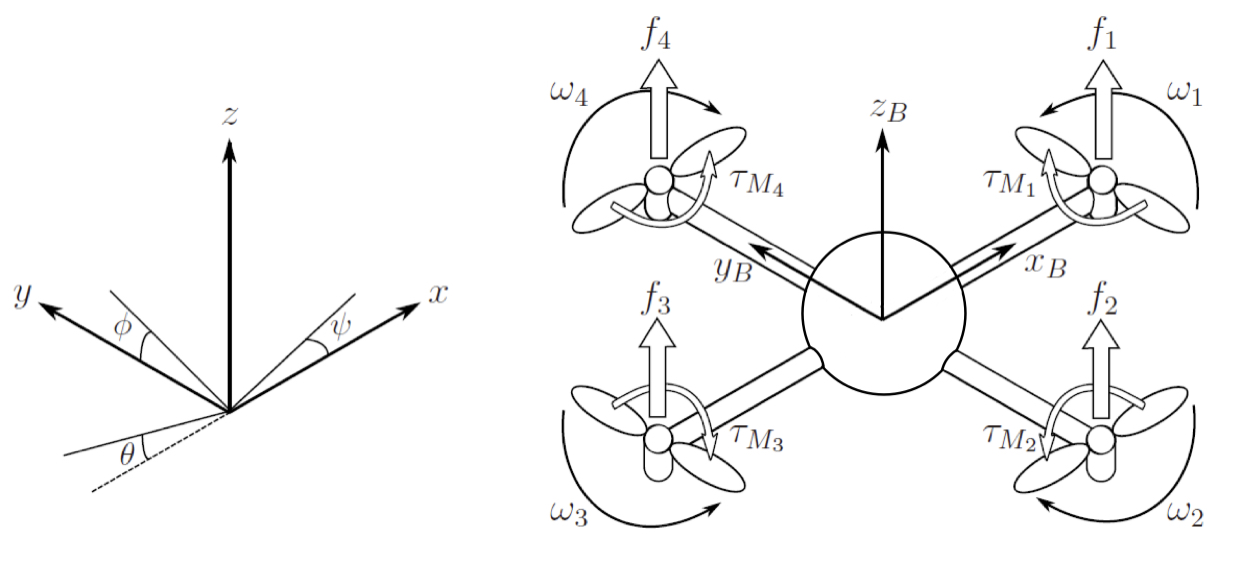
\includegraphics[width= 0.7\linewidth, angle %=0]{Images/Model.png}
%\caption{The simplified frame for a quadcopter.}
%\label{fig:1}
% %\end{figure}

% ...
% \begin{itemize}

% \item  Formulate the problem (do not simply copy the problem description).
% \item  Include any references to this problem (or a very similar one) you may have found in the literature (acknowledge any references!, see 5.). Here are examples of references \cite{kittel05}. For details please see the attached \LaTeX file \cite{ashcroft02}.
% \item Highlight the laws of physics behind the problem;
% \item Argue for the approach you will be using;
% Formulation of the model: here you should clearly formulate all assumptions, hypotheses and introduced variables.  You should also point out why you choose this model.
% \item You may include a sketch/figure/graph if it is necessary to explain your model.

% \end{itemize}